\documentclass{article}
\usepackage{listings}
\usepackage{graphicx}
\graphicspath{ {images/} }
\usepackage{times}
\usepackage{url}
\usepackage{hyperref}
\hypersetup{colorlinks=true}
\title{Binary Search Trees}
\author{Scurtu Estera Daniela }
\date{\today}
\begin{document}
\maketitle
Grupe 10106B

1st year

Computer and Information Technology(English) 
\pagebreak
\section{Problem statement}

A library for binary search trees (BST). 

The library should provide operations for: creating an empty tree, inserting a node into a tree, deleting a node and at least two different traversal strategies; the traversal functions must accept a function which will be passed the current element.

\section{Application Design}
Binary Search Tree, is a node-based binary tree data structure which has the following properties:
\begin{itemize}
\item The left sub-tree of a node contains only nodes with keys less than the node’s key.
\item The right sub-tree of a node contains only nodes with keys greater than the node’s key.
\item The left and right sub-tree each must also be a binary search tree.
\item There must be no duplicate nodes.
\end{itemize}

Binary Search Tree can be implemented as a linked data structure in which each node is an object with two pointer fields and an information field. The two pointer fields left and right point to the nodes corresponding to the left child, right child. NULL in any pointer field signifies that there exists no corresponding child. 

\subsection{Inputs}

Input data is read from a file named test.in.txt which has the following structure: 
\begin{itemize}
    \item the first line contains the number of nodes that are initially in the tree
    \item the second line contain the number of tests to be made
    \item the next nrTeste lines, has each two values, one for the nodes to be inserted in the tree and one for the nodes to be deleted from the tree.
\end{itemize}

Here is an example of inputs for this algorithm:
\input{test.in.txt}
\subsection{Outputs}

First output is the number of nodes of the tree followed by a traversal of the tree, breadth first tree traversal. The rest output consists in nrTeste tests which include inserting nrNodeAdd in the tree and deleting nrNodeDel from the tree.

This image is a part of output, the test number 5. 

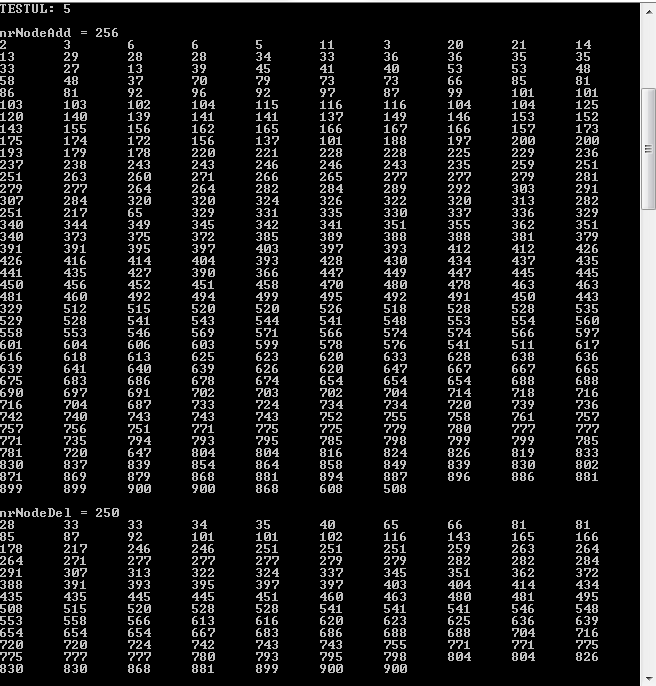
\includegraphics[scale=0.69]{test5}

If we were to run again the program, the numbers would be different because the program would generate different numbers for each run.

\indent \indent \indent  \indent
\subsection{Operations on Binary Search Trees}
\begin{enumerate}
\item Create an element

\begin{quotation}
This operation can be seen in the procedure "getNode" which have a parameter of type int, that represent the value we want to store in the created node. Firstly I allocate memory for one element of type "bstNode" using the "malloc" function, next step is to store the value key in the data field. The last step to be taken is to initialize the right and left fields of the node to NULL.

I will use this function in the procedure "insert\_bst" to create the node to be inserted in the tree.
\end{quotation}
\item Insertion of a node in the tree
\begin{quotation}
For this operation I used a function named "insert\_bst" with two parameters one of type bstNode which is the adress of the root, and an integer which represents the value to be inserted. Insertion begins as a search would begin; if the key is not equal to that of the root,
we search the left or right subtrees as before. Eventually, we will reach an external node and add the new key-value pair  as its right or left child, depending on the node's key. In other words, we examine the root and recursively insert the new node to the left subtree if its key is less than that of the root, or the right subtree if its key is greater than or equal to the root
\end{quotation}
\item Deletion of a node of the tree
\begin{quotation}
This operation is described in the procedure "deleteNode" with two parameters, one that represent the adress of the root and another one that takes the value to be deleted. Deletion also begins as a search, we try to find where the node that has the value we want to delete is, if the key is lesser than the root(the actual node) value we use recursion and call the function to move in the left sub-tree and take the steps from the beginning, else if is greater we move in the right sub-tree, else we find the wanted value and from here three cases can be distinguished:
\begin{itemize}
\item Case 1: the node has no child - this case is the simple one because the wanted node already points to NULL so all we have to do is to deallocate the node using the function free and make it NULL.
\item Case 2: the node has one child - here there can be two cases, the node can have either the left child or the right child. If the node has only a left child, we put all the left sub-tree int the place of the node to be deleted. I made this using an auxiliary variable named temp which will copy the address of the root, and make the root point to its left child, while the auxiliary variable will be deallocated. The case for the right child is similar the only difference is where the root node will point.
\item Case 3: the node has two children - to solve this case I will use a function "findMin" which goes to the most left child of the tree, which is the minimum value and return its address. I will use the auxiliary variable again, this time it will store the address of the minimum value in the right sub-tree, we copy this value to the node we want to delete. Now there will be two nodes that store the same value, because we don't know in which one of the cases we are we will call the function with the parameters root->right and root->data, which is the minimum value in the right sub-tree.
\end{itemize}
\end{quotation}
\item Traversal of a tree.

There are two known types of traversal for a Binary Search Tree:
\begin{enumerate}
    \item Depth First Search which can be
        \begin{itemize}
            \item Pre-order Traversal 
            \item In-order Traversal
            \item Post-order Traversal
        \end{itemize}
            
    \item Breadth First Search - to implement this traversal we will use three functions which take as a parameter the address of the root: "height" which compute the height of the tree the number of
    nodes along the longest path from the root node
    down to the farthest leaf node, "printGivenLevel" which print the node of a given level, "level" is a parameter of the procedure and the last function is printLevelOrder print all the nodes in level order.
\end{enumerate}
\item Search for a given value in the tree 

\begin{quotation}
The procedure for this task is named "search\_node" and takes two parameters, one of type bstNode, which is the adress of the root, and one integer which is the value we want to find. First we compare the given value with the data stored in the node, if it is greater than the node's data we move the search in the right subtree, else we are looking for the value in the left sub-tree. Once we find the value we retuen its adress.
\end{quotation}
\item Add elements in the tree
\begin{quotation}
The procedure used for this operation is create\_bst. This function use the function radomize which generate random numbers that are inserted in the tree using the insert\_bst function. To prevent the insertion of the same number I used the goto function which force the algorithm to reread a number if it exists in the tree. 
\end{quotation}
\item Delete elements from the tree
\begin{quotation}
The procedure used for this operation is nodeDelete. This function generate random numbers which are delete from the tree using the deleteNode function. Because I can not know which are the current numbers of the tree and also the numbers generated randomly I check if the data is in the tree first, if it is it will be deleted, it it is not the program will generate another number to be deleted.
\end{quotation}
\end{enumerate}
\indent  \indent   \indent    \indent  \indent   \indent  \indent

\section{Pseudocode}
\begin{itemize}
    \item The procedure insert\_bst
\end{itemize}

procedure insert\_bst (var root :struct bstNode; 

\indent  \indent   \indent    \indent  \indent   \indent  \indent
  var key : integer) : struct bstNode
  
  
1.\indent  begin

2.\hspace{40pt} {\bf if} root = NULL {\bf then}

3.\hspace{50pt} root := getNode(var root ; var key)

4.\hspace{40pt} end

5.\hspace{40pt} else if $root\rightarrow data < key$ \hspace{5pt} then

6.\hspace{50pt} $root\rightarrow left$ := $insert\_node(root\rightarrow left, key)$

7.\hspace{40pt} end

8.\hspace{40pt} else if $root\rightarrow data > key$ \hspace{5pt} then

7.\hspace{50pt} $root\rightarrow right$ := $insert\_node(root\rightarrow right, key)$

8.\hspace{40pt} end

9.\hspace{40pt} return root

10.\hspace{30pt} end insert\_node
\begin{itemize}
    \item The procedure deleteNode
\end{itemize}

procedure deleteNode (var root :struct bstNode; 

\indent  \indent   \indent    \indent  \indent   \indent  \indent
  var key : integer) : struct bstNode
  
1.\hspace{30pt} begin

2.\hspace{40pt} var temp : bstNode

3.\hspace{40pt} if $root$ = $NULL$ \hspace{5pt} then

4.\hspace{50pt} return root;

5.\hspace{40pt} end

6.\hspace{40pt} if $root\rightarrow data < key$ \hspace{5pt} then

7.\hspace{50pt} $root\rightarrow left$ := $deleteNode(root\rightarrow left, key)$

b.\hspace{40pt} end

9.\hspace{40pt} else if $root\rightarrow data > key$ \hspace{5pt} then

10.\hspace{50pt} $root\rightarrow right$ := $deleteNode(root\rightarrow right, key)$

11.\hspace{40pt} end

12.\hspace{40pt} else if ! $root\rightarrow left$ \hspace{5pt} and \hspace{5pt}  ! $root\rightarrow right$ \hspace{5pt}then

13.\hspace{50pt} free root

14.\hspace{50pt} root := NULL 

15.\hspace{40pt} end

16.\hspace{40pt} else if $root\rightarrow left$ =$ NULL$ \hspace{5pt} then

17.\hspace{50pt} $temp$ := $root$

18.\hspace{50pt} $root$ := $root\rightarrow right$

19.\hspace{50pt} free temp

20.\hspace{40pt} end

21.\hspace{40pt} else if $root\rightarrow left $= $NULL$ \hspace{5pt} then

22.\hspace{50pt} $temp$ :=$ root$

23.\hspace{50pt} $root$ := $root\rightarrow right$

24.\hspace{50pt} free temp

25.\hspace{40pt} end

26.\hspace{40pt} else if $root\rightarrow left$ \hspace{5pt} and \hspace{5pt} $root\rightarrow right$ then

27.\hspace{50pt} $temp $:= $findMin (root\rightarrow right)$

28.\hspace{50pt} $root\rightarrow data$ := $temp\rightarrow data$

29.\hspace{50pt} $root\rightarrow right$ := $deleteNode(root\rightarrow right, root\rightarrow data)$

30.\hspace{40pt} end

31.\hspace{30pt} end deleteNode

\begin{itemize}
    \item The procedure search\_node
\end{itemize}

procedure search\_node (var root :struct bstNode; 

\indent  \indent   \indent    \indent  \indent   \indent  \indent
  var key : integer) : struct bstNode
  
  
1.\indent  begin

2.\hspace{40pt} {\bf if} root = NULL {\bf then}

3.\hspace{50pt} return false

4.\hspace{40pt} end

5.\hspace{40pt} if $root\rightarrow data = key$ \hspace{5pt} then

6.\hspace{50pt} return true

7.\hspace{40pt} end

8.\hspace{40pt} else if $root\rightarrow data < key$ \hspace{5pt} then

9.\hspace{50pt} return $search\_node(root\rightarrow left, key)$

10.\hspace{40pt} end

11.\hspace{40pt} else if $root\rightarrow data > key$ \hspace{5pt} then

12.\hspace{50pt} return $search\_node(root\rightarrow roght, key)$

13.\hspace{40pt} end

14.\hspace{30pt} end insert\_node
\section{Conclusions}
\hspace{10pt}Only using linked lists may not be enough in some applications, for example if we want a description of a product, we would need an hierarchical description of its components. Hierarchical organisation of data is used in various fields and we can say that every physical entity can be represented as trees.
The binary search tree is a different way of structuring data in hierarchical way so that it can still be binary searched (or a very similar procedure can be used), but it's easier to add and remove elements.
The implementation based on dynamic programming makes the code clear and easily understandable and reduce the complexity of the algorithm.

The algorithm I made presents the most important operations that can be made on binary search trees, operations like insertion, deletion, traversals and binary search. The most challenging part of the project was to write the procedure for deletion because it is very complex and it took a lot of time to realise which was my mistake.  

\section{References}
\begin{thebibliography}{9}

	\bibitem{ellis}
	  Sara Baase, Computer Algorithms, Introduction to Design and Analysis 
	  \emph{Edison-Wesley Publishing Company}.
	  Edison Wesley,
	  2nd Edition,
	  
    \bibitem{ellis}
	  Ellis Horowitz, Fundamentals of Programming Languages, 
	  \emph{Computer Science Press}.
	  Computer Science Press,
	  2nd Edition,

    \bibitem{bst}
     site 
     url {http://www.geeksforgeeks.org/category/binary-search-tree/},.

\end{thebibliography}
\section{Source Code}
Here are all the function I described above implemented in C
\begin{lstlisting}
#ifndef BST_H_H_INCLUDED
#define BST_H_H_INCLUDED
#include "bst_c.c"

struct bstNode *getNode(int key);

struct bstNode *insert_bst(struct bstNode *root,int key);

bool search_node(struct bstNode *root, int key);

struct bstNode *create_bst(struct bstNode *root, int nrNode);

int bstSrd(struct bstNode *root);

int bstRsd(struct bstNode *root);

int bstSdr( struct bstNode *root);

struct bstNode *findMin(struct bstNode *root);

struct bstNode *deleteNode(struct bstNode *root, int key);

int printGivenLevel(struct bstNode* root, int level);

int height(struct bstNode* root);

void printLevelOrder(struct bstNode* root);

void freeTree(struct bstNode *root);

void nodeDelete(struct bstNode *root, int n);
#endif // BST_H_H_INCLUDED

\end{lstlisting}

\begin{lstlisting}

#include <stdio.h>
#include <stdlib.h>
#include <stdbool.h>
#include <time.h>
#include "bst_h.h"
int randomize();
struct bstNode{

    int data;               
    struct bstNode *left; 
    struct bstNode *right;  
};
struct bstNode *getNode(int key){
    struct bstNode *node = (struct bstNode *) malloc( sizeof ( struct bstNode));
    node->data = key;
    node->left = node->right = NULL;
    return node;
}

struct bstNode *insert_bst(struct bstNode *root, int key){
    if(root == NULL){
        root = getNode(key);
    }
    else if( key < root->data){
        root->left = insert_bst( root->left, key);
    }
    else{
        root->right = insert_bst( root->right, key);
    }
    return root;
}

bool search_node(struct bstNode *root, int key){
    if(root == NULL){
        return false;
    }
    else if( root->data == key){
        return true;
    }
    else if(key < root->data){
        return search_node(root->left, key);
    }
    else{
        return search_node(root->right, key);
    }
}

struct bstNode *create_bst(struct bstNode *root, int nrNode){
    int i, data;
    for( i = 0; i < nrNode; i++){
pas0:   data = rand() % 900 + 1;
        if(search_node(root,data)){
            goto pas0;
        }
        else{
            root = insert_bst(root, data);
        }
    }
}

int bstSrd(struct bstNode *root){

    if( root == NULL){
            return 0;
    }
    bstSrd(root->left);
    printf("%d\t", root->data);
    bstSrd(root->right);

}

int bstRsd(struct bstNode *root){
    if(root == NULL){
            return 0;
    }
    printf("%d\t", root->data);
    bstRsd(root->left);
    bstRsd(root->right);
}

int bstSdr( struct bstNode *root){
    if(root == NULL){
            return 0;
    }
        bstSdr(root->left);
        bstSdr(root->right);
        printf("%d\t",root->data);

}

int height(struct bstNode* root)
{
    if (root==NULL)
        return 0;
    else
    {
/** compute the height of each subtree */
        int leftHeight = height(root->left);
        int rightHeight = height(root->right);

/** use the larger one */
        if (leftHeight > rightHeight){
            return(leftHeight+1);
        }
        else{
                return (rightHeight+1);
        }
    }
}

int printGivenLevel(struct bstNode* root, int level)
{
    if (root == NULL)
        return;
    if (level == 1)
        printf("%d\t", root->data);
    else if (level > 1)
    {
        printGivenLevel(root->left, level-1);
        printGivenLevel(root->right, level-1);

    }
}

void printLevelOrder(struct bstNode* root)
{
    int h = height(root);
    int i;
    for (i=1; i<=h; i++){
        printGivenLevel(root, i);

    }
}

struct bstNode *findMin(struct bstNode *root){
    if(root == NULL){
        printf("the tree is empty");
        return 0;
    }
    else if( root->left == NULL){
        return root;
    }

    return findMin(root->left);
}

struct bstNode *deleteNode(struct bstNode *root,int key) {
    struct bstNode * temp;
    if (root == NULL) {
        return root;
    }
    if (key < root->data) {
        root->left = deleteNode(root->left, key);
    }
    else {
        if(root->left == NULL && root->right == NULL){
            free(root);
            root = NULL;
        }
        else if (root->left == NULL) {
                temp = root;
                root = root->right;
                free(temp);
        }
        else if (root->right == NULL) {
                    temp = root;
                    root = root->left;
                    free(temp);
            }
        else if (root->left != NULL  && root->right != NULL) {
                temp = findMin(root->right);
                root->data = temp->data;
                root->right = deleteNode(root->right, root->data);
            }
        }

    return root;
}

void freeTree(struct bstNode *root) {
    if (root == NULL) {
        return;
    }
    freeTree(root->left);
    freeTree(root->right);
    free(root);
}

void nodeDelete(struct bstNode *root, int n){
    int i;
    int data;
    for(i = 0; i < n; i++ ){
pas1:   data = rand() % 900;
        if(search_node(root,data)){
            root = deleteNode(root, data);
        }
        else{
            goto pas1;
        }
    }
}

\end{lstlisting}
\begin{lstlisting}
#include "bst_h.h"
int main()
{
    srand(time(NULL));
    FILE *test;     
    test = fopen("test.in.txt","r");
    
    int nrTeste;
    int nrNode;
    int nrNodeAdd;
    int nrNodeDel;

    struct bstNode *root = NULL;
    root = insert_bst(root, 500);

    fscanf(test,"%d",&nrNode);
    fscanf(test,"%d",&nrTeste);
    printf("Numarul de elemente din arbore este %d\n",nrNode);
    create_bst(root, nrNode);
    printLevelOrder(root);
    printf("\n\n\n");
    while(nrTeste != 0){
        printf("\n\nTESTUL: %d\n ",nrTeste);
        fscanf(test,"%d %d",&nrNodeAdd, &nrNodeDel);
        printf("\nnrNodeAdd = %d\n", nrNodeAdd);
        create_bst(root, nrNodeAdd);
        bstSdr(root);
        printf("\n\nnrNodeDel = %d\n",nrNodeDel);
        nodeDelete(root,nrNodeDel);
        bstSrd(root);

        nrTeste--;

    }
    freeTree(root);
    fclose(test);
}

\end{lstlisting}

Here is the code in Python3.5 for the algorithm. I must say that this code does not work entirely, it is a problem when trying to delete more numbers. I tried to fix this problem but I could not do that.

\begin{lstlisting}
class Node:
    def __init__(root, val):
        root.right = None
        root.left = None
        root.data = val

def insert(root, data):
    if root.data:
        if data < root.data:
            if root.left is None:
                root.left = Node(data)
            else:
               insert(root.left,data)
        elif data > root.data:
            if root.right is None:
                root.right = Node(data)
            else:
                insert(root.right, data)
    else:
        root.data = data

def SRD(root):
    if root is None:
        return
    SRD(root.left)
    print (root.data)
    SRD(root.right)

def RSD(root):
    if root is None:
        return
    print (root.data)
    RSD(root.left)
    RSD(root.right)

def bin_search(root, data):
    if root is None:
        return 0
    elif root.data is data:
        return 1
    elif data < root.data:
        return bin_search(root.left,data)
    else:
        return bin_search(root.right,data)

def find_min(root):
    if root is None:
        print ("the tree is empty")
        return
    elif root.left is None:
        return root
    return find_min(root.left)

def delete_node(root, data):
    if root is None:
        return root 
    if data < root.data:
        root.left = delete_node(root.left, data)
    elif data > root.data:
        root.right = delete_node(root.right, data)
    else:
        if root.left is None and root.right is None:
            del root
            root = None
        if root.left is None :
            temp = root.right 
            root = None
            return temp       
        elif root.right is None :
            temp = root.left 
            root = None
            return temp
        temp = find_min(root.right)
        root.data = temp.data
        root.right = delete_node(root.right , temp.data)
    return root

def create_bst(root,n):
   for i in range (1,n):
       a = randint(0,300)
       insert(root,a)

def delete_bst(root,n):
   for i in range (1,n):
       a = randint(0,300)
       delete_node(root,a)
       

from random import randint
root = Node(110)
create_bst(root,150)
SRD(root)
delete_bst(root,50)
RSD(root)
\end{lstlisting}
\section{Experiments and results}
To check the correctness of the algorithm I made 6 tests, each consisting in inserting a number of nrNodeAdd nodes in the tree and deleting a number nrNodeDel from the tree, the nrNodeAdd and nrNodeDel are two variables read from a file. The results were displayed using three traversal functions: level order traversal, to display the initial tree, in-order traversal, to print the tree after the insertion and post-order traversal for printing the remaining nodes after deletion.
\end{document}
